%\documentclass[a4paper,10pt]{article}
\documentclass[a4paper,10pt,twocolumn]{article}
\usepackage[utf8]{inputenc}

\usepackage{graphicx}
\usepackage{float}
\graphicspath{ {images/} }


%opening
\title{Rigid Motions and Homogeneous Transformations}
\author{Erivelton Gualter}

\begin{document}

\date{}
\maketitle


\section*{Chapter 2}

\textbf{Homogeneous transformations} combine the operations of rotation and translation into a single matrix multiplication.

\begin{figure}[H]
\centering
 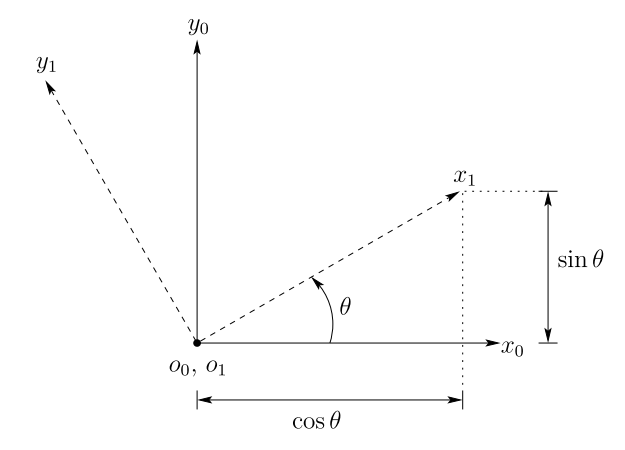
\includegraphics[width=0.8\linewidth]{ch2-coordinate.png}
\end{figure}

$R^0_1$ : Coordinate vectors for the axes of frame $o_1x_1y_1$ with respect to coordinate frame $o_0x_0y_0$:

\begin{figure}[H]
\centering
 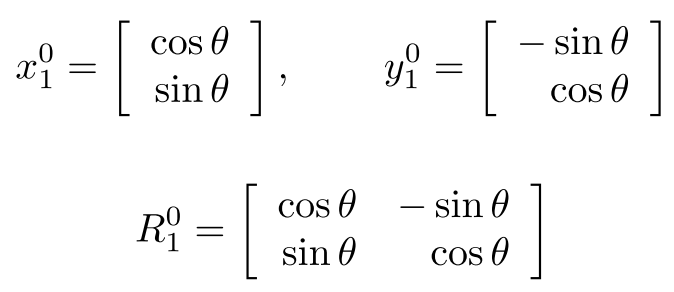
\includegraphics[width=.7\linewidth]{Rotation2D.png}
 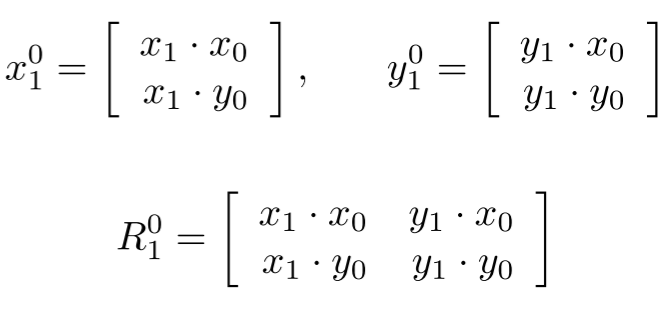
\includegraphics[width=.7\linewidth]{Rotation2D2.png}
\end{figure}

\textbf{Rotation in Three Dimensions}

\begin{figure}[H]
\centering
 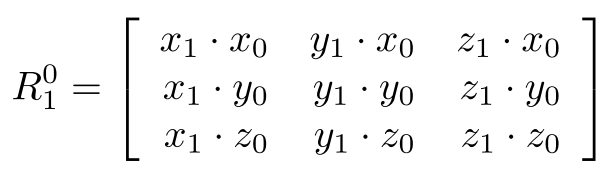
\includegraphics[width=0.6\linewidth]{rotation3d.png}
\end{figure}

Remember: If $u$ is parallel to $v$, $u \cdot v = 1$. Also, if $u$ is perpendicular to $v$, $u \cdot v = 0$.

\begin{itemize}
 \item Rotations relative to the current frame (recursively defined); or rotations relative to a fixed frame (usually the world frame).
\end{itemize}

\begin{figure}[H]
\centering
 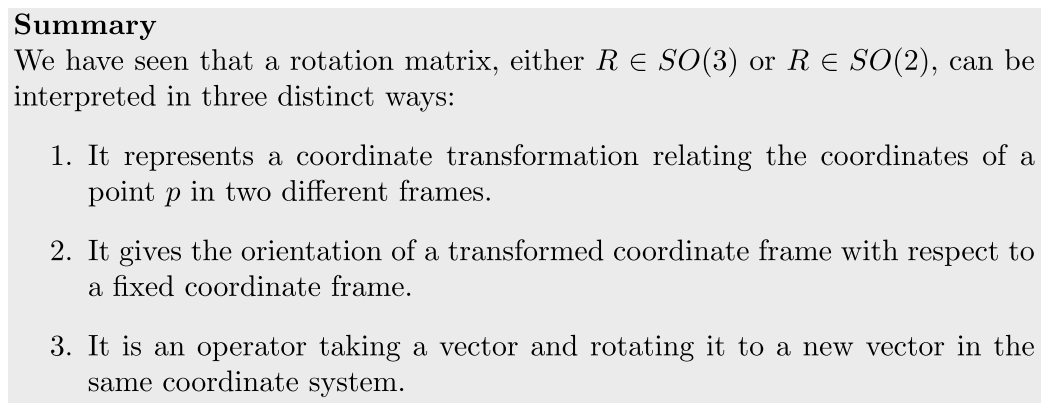
\includegraphics[width=1\linewidth]{summaryRotation.png}
\end{figure}


\begin{figure}[H]
\centering
 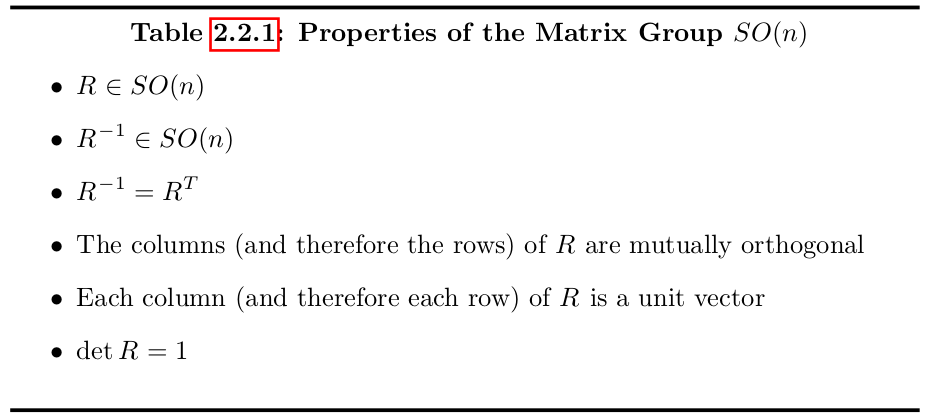
\includegraphics[width=1\linewidth]{ch2-tables.png}
\end{figure}

Example of Composition of Rotational Transformations:
\begin{figure}[H]
\centering
 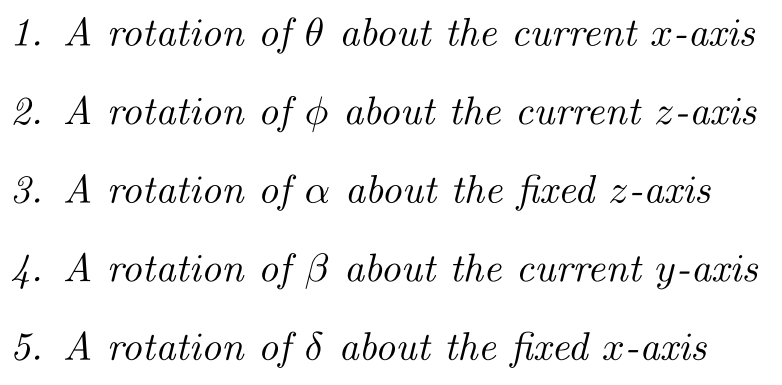
\includegraphics[width=.8\linewidth]{ex2_8.png}
\end{figure}

\begin{figure}[H]
\centering
 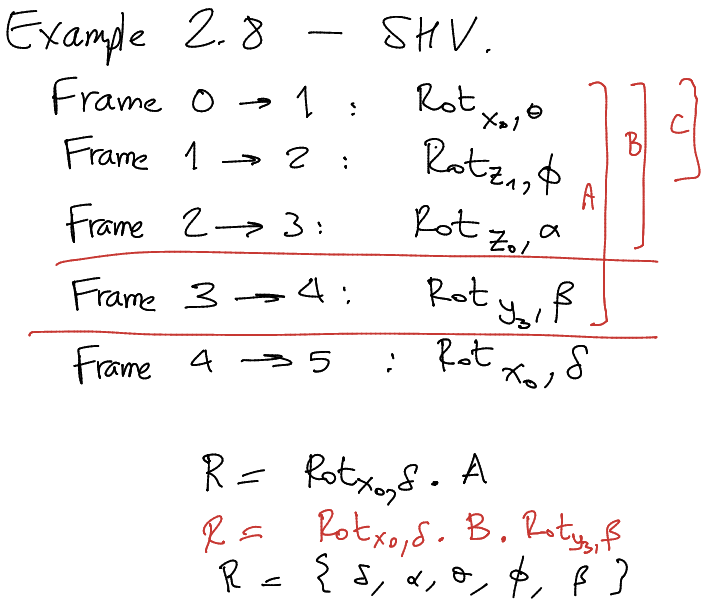
\includegraphics[width=.8\linewidth]{rotatiodecomposition.png}
\end{figure}


\section*{Chapter 3}

\begin{itemize}
 \item \textbf{Forward Kinematics}: Determine the position and orientation of the end effector given the values for the joint variables of the robot. Also known as \textit{configuration kinematics}.
 \item \textbf{Inverse Kinematics}: Determine the values of the joint variables given the end effector's position and orientation.
\end{itemize}

\subsection*{Kinematic Chains}

Robot manipulator is composed of a set of links connected together by joints. Each joint has a sigle degee-of-feedom of motion. For instance, the \textbf{angle of rotation} for revolute joint and \textbf{linear displacement} for a prismatic joint.

\begin{itemize}
 \item Robot manipulator with \textit{n} joints have $n+1$ links.
 \item Joints numbering: $1$ to $n$.
 \item Links numbering: $0$ to $n$ starting from the base.
 \item Joint $i$ connects link $i-1$ to link $i$.
 \item WHen joint $i$ is actuated, link $i$ moves.
 \item Joint variable $q_i$: When $i$ correspond to the revolute joint $q_i = \theta_i$. When $i$ correspond to prismatic joint $q_i = d_i$.
 $$ q_i=\left\{\begin{array}{cc} \theta_i & \textrm{revolute joint}\\ d_i & \textrm{prismatic joint} \end{array} \right. $$
\end{itemize}

\textbf{Homogeneous Transformation Matrix}: Expresses the position and orientation of $o_jx_jy_jz_j$ with respect to $o_ix_iy_iz_i$: ($T^i_j$).

\begin{figure}[H]
\centering
 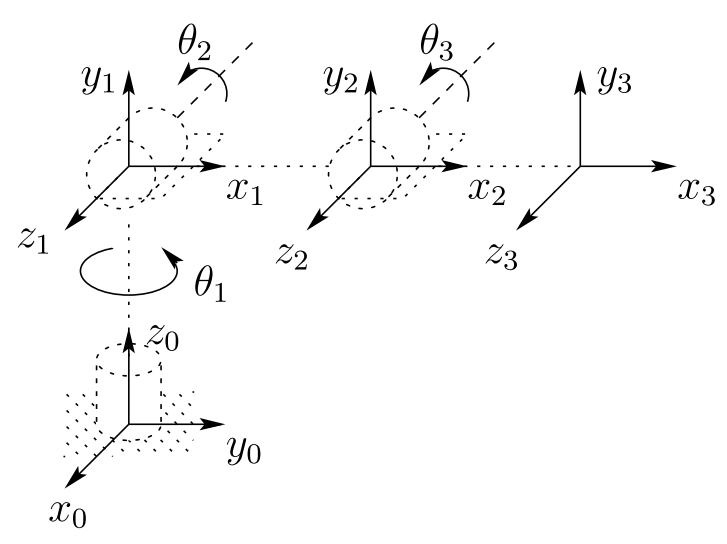
\includegraphics[width=0.8\linewidth]{elbowManipulator.png}
\end{figure}

\subsection*{The Denavit-Hartenberg Convention or DH convention}

Each Transformation $A_i$ is represented as a product of four basic transformations:

\begin{figure}[H]
\centering
 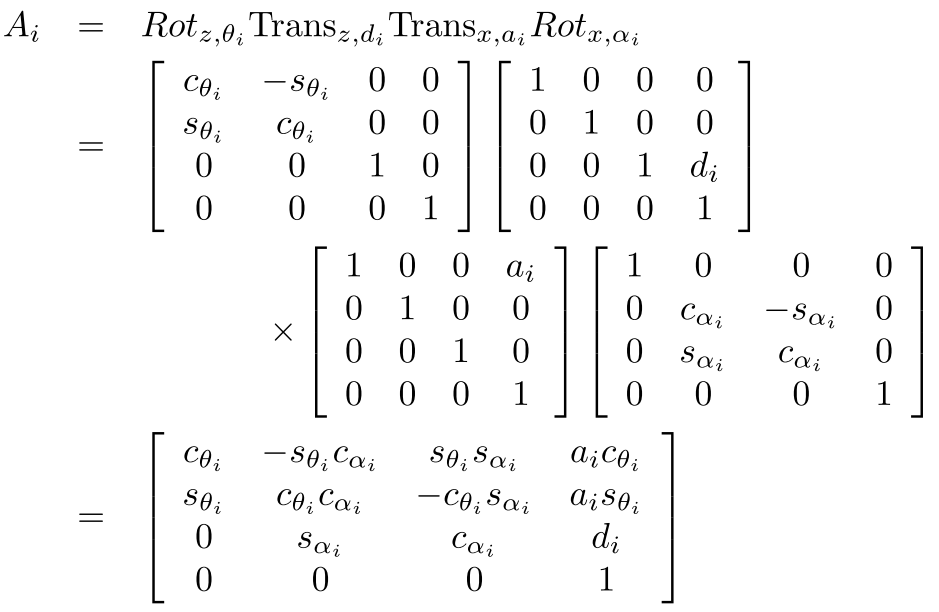
\includegraphics[width=1\linewidth]{HomTransDH.png}
\end{figure}

where: $\theta_i$, $a_i$, $d_i$, $\alpha_i$ correspond to the joint angle, link length, link offset, and link twist.

\begin{figure}[H]
\centering
 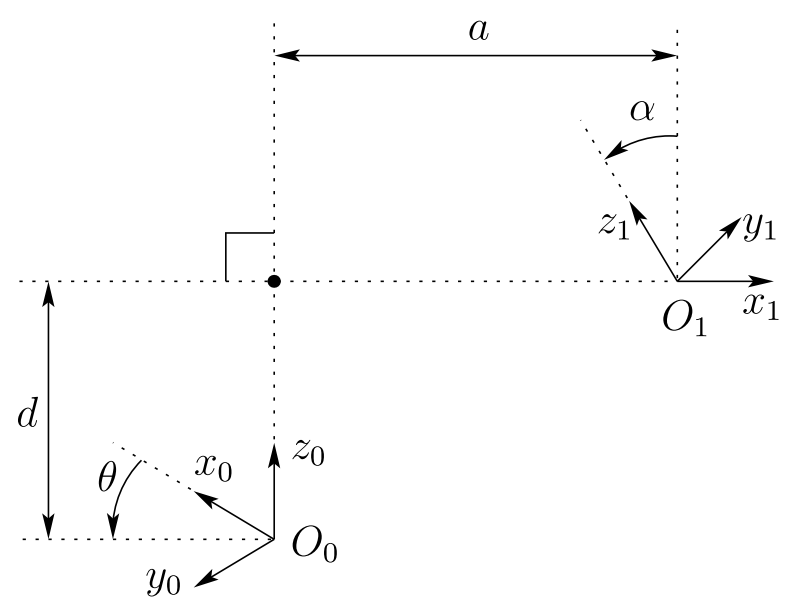
\includegraphics[width=0.8\linewidth]{assumptionsDH.png}
\end{figure}

\begin{figure}[H]
\centering
 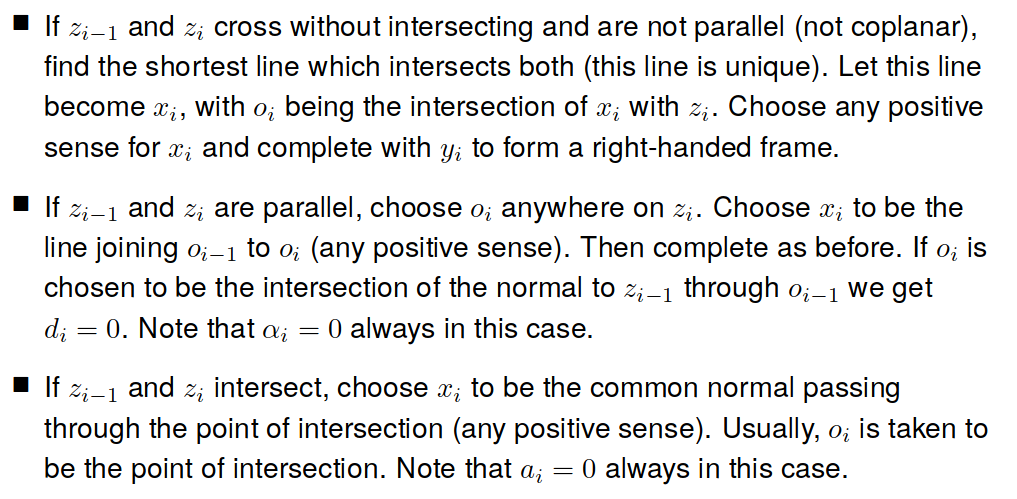
\includegraphics[width=1\linewidth]{ThreeCasesDH.png}
 \caption{Hanz Richter's notes.}
\end{figure}


\subsection*{Inverse Kinematics}

Goal: Find the \textbf{joint variables} in terms of the end-effector position and orientation.



\end{document}
